\section{Related Work}
Bevor auf Tensorflow genauer eingegangen wird, soll dieses Kapitel eine Übersicht über folgende Deep Learning Frameworks geben:
\begin{multicols}{2}
	\begin{itemize}
		\item Torch
		\item Caffe
		\item Caffe2
		\item Keras
		\item Chainer
		\item \acs{cntk}
		\item Apache MXNet
		\item Amazon \acs{dsstne}
		\item Eclipse \acl{dl4j}
	\end{itemize}
\end{multicols}
	
\subsection{Torch}
Torch wurde ursprünglich von Facebook entwickelt und 2017 als Open-Source Projekt veröffentlicht. Das Framework bietet zwei Hauptfunktionen: Erstens, mathematische Berechnung unter starker Unterstützung der \ac{gpu}. Dabei wird es oft als Ersatz für das bekannte Python Framework Numpy eingesetzt, da es durch die \ac{gpu}-Unterstützung eine wesentlich bessere Performance bietet. Zweitens, zur Bildung von neuronale Netze für Deep Learning, dabei wirbt das Framework mit maximaler Flexibilität und Geschwindigkeit \cite{Torch}. Laut DL4J zeichnet sich das Framework durch viele Modulare Funktionen aus, die sich einfach kombinieren lassen. Des Weiteren lassen sich einfach neue Layer definieren und auf der GPU ausführen. Jedoch bietet Torch keinen kommerziellen Einsatz und die Dokumentation soll nicht vollständig sein \cite{DeepLearningFrameworks}. 

\subsection{Caffe}
Caffe ist ein Open-Source Projekt, das von Yangqing Jia im Rahmen seiner Doktorarbeit beim \ac{bair} initiiert wurde. Aktuell wird es vom \ac{bair} und Community Entwicklern weiterentwickelt. Mit nur wenigen Zeilen Code lassen sich Modelle erstellen, dabei lässt sich konfigurieren ob die Berechnungen auf der \acs{cpu} oder \ac{gpu} durchgeführt werden. Caffe wird hauptsächlich zur Verarbeitung von Bildern eingesetzt und kann mit nur einer \ac{gpu} über 60 Millionen Bilder pro Tag verarbeiten \cite{Caffe}. Aktuell bietet Caffe noch keine Möglichkeit die Berechnung verteilt von mehreren \ac{gpu} durchzuführen \cite{DeepLearningFrameworks}.

\subsection{Caffe2}
Der Erfinder von Caffe Yangqing Jia arbeitet jetzt bei Facebook und entwicklte dabei an einer Erweiterung von Caffe. Diese wurde unter dem Name Caffe2 veröffentlicht und bietet mehr Skalierbarkeit und Leichtgewichtigkeit gegenüber Caffe. Zudem erlaubt Caffe2 das Verteilen von Aufgaben bzw. Berechnung auf mehrere Instanzen \cite{Caffe2}.

\subsection{Keras}
Keras ist ein High-Level \ac{api} für neuronale Netze und basiert auf Tensorflow, welches in Kapitel \ref{sec:tensorflow} genauer erläutert wird. Die Entwicklung von Keras folgte dem Motto: "Die Fähigkeit, mit möglichst wenig Verzögerung von der Idee zum Ergebnis zu kommen, ist der Schlüssel für eine gute Forschung" \cite{Keras}. Somit ermöglicht Keras das schnell aufsetzen und testen von Neuronalen Netzen. Elephans ist eine Erweiterung für Keras, die das verteilen einer Anwendung über mehrerer Instanzen erlaubt \cite{Elephas}.

\subsection{Chainer}
Chainer ist auch ein Open-Source Deep Learning Framework und bietet ein flexibles, intuitives und leistungsstarkes Mittel zur Implementierung einer ganzen Reihe von Deep-Learning-Modellen, einschließlich State-of-the-Art-Modellen wie z. B. rekurrenten neuronalen Netzen und variationalen Autoencodern. Mit Chainer können Anwendungen auf mehrere Instanzen verteilt werden und dadurch wie in Abbildung \ref{fig:chainercomparisson} zu sehen im Bereich Performance andere Frameworks klar hinter-sich lassen. Die optimale Performance wurde beim verteilen einer Anwendung auf 128 \ac{gpu}s erreicht \cite{Chainer}.

\begin{figure}[h!]
	\centering
	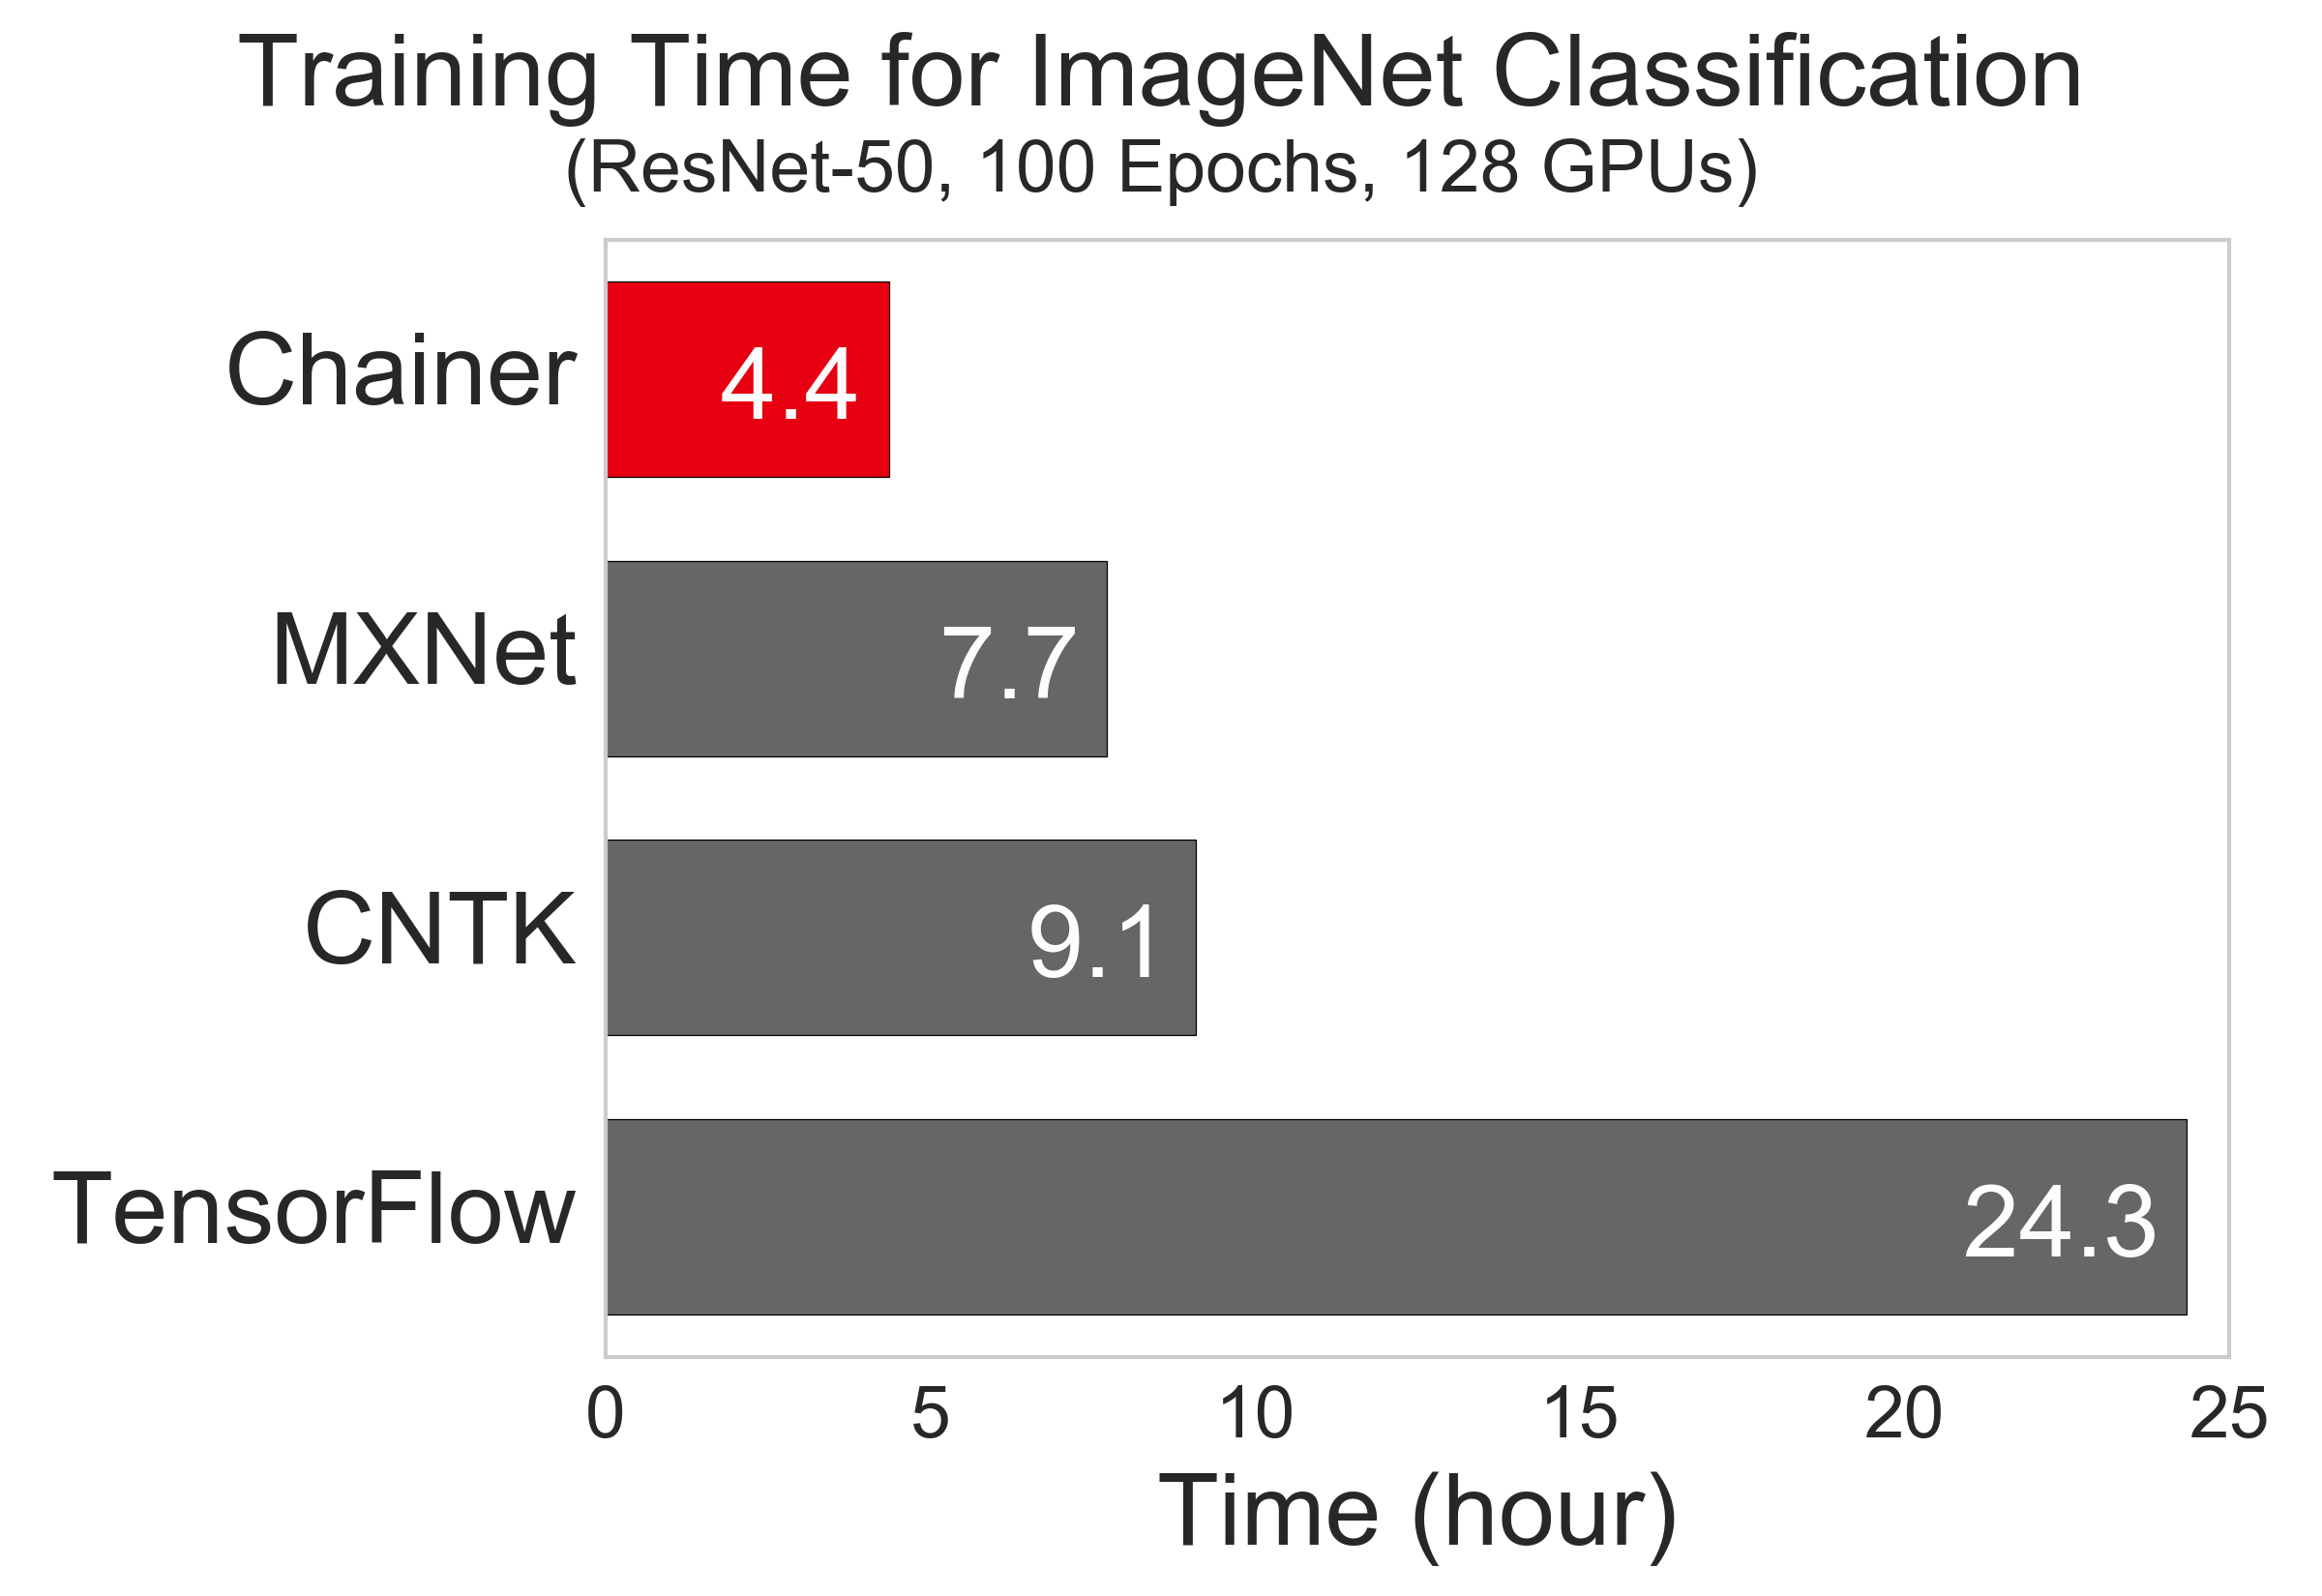
\includegraphics[width=0.9\linewidth]{Pictures/Chainer_Comparisson}
	\caption[Deep Learning Framework Vergleich]{Deep Learning Framework Vergleich \cite{Chainer}}
	\label{fig:chainercomparisson}
\end{figure}

\subsection{\acf{cntk}}
\ac{cntk} ist ein Open-Source Framework für das verteilen einer Deep-Learning Anwendung im kommerziellen Bereich. Es beschreibt neuronale Netze als eine Reihe von Rechenschritten über einen gerichteten Graphen. \ac{cntk} erlaubt dem Benutzer, populäre Modelltypen wie feed-forward DNNs, konvolutionelle neurale Netze (CNNs) und wiederkehrende neurale Netze (RNNs / LSTMs) leicht zu verwirklichen und zu kombinieren. \ac{cntk} implementiert stochastisches Gradientenabstiegsverfahren (SGD, Error Backpropagation) mit automatischer Differenzierung und Parallelisierung über mehrere \ac{gpu}s und Server hinweg \cite{CNTK}.

\subsection{Apache MXNet}
Apache MXNet ist ein modernes Open-Source Deep Learning Framework, mit dem neuronale Netze trainiert und implementiert werden können. Es ist skalierbar, ermöglicht schnelles Modelltraining und unterstützt ein flexibles Programmiermodell und mehrere Programmiersprachen. Die MXNet-Bibliothek ist portabel und kann auf mehreren \ac{gpu}s und mehreren Instanzen skaliert werden. MXNet wird von den wichtigsten Public Cloud-Anbietern wie \ac{aws} und Azure unterstützt \cite{WikipediaApacheMXNet}. Amazon und Microsoft arbeiteten zusammen an einer \ac{api} für Apache MXNet und veröffentlichten im Oktober 2017 Gluon, eine neue Open-Source Deep-Learning Schnittstelle, die es Entwicklern ermöglicht, einfach und schnell Machine-Learning-Modelle zu erstellen, ohne dabei die Leistung zu beeinträchtigen \cite{AWSintroducingGluon}.

\subsection{Amazon \acs{dsstne}}
Amazon \ac{dsstne} ist eine Open-Source Deep Learning Framework zum entwicklen von Empfehlungsmodellen. \ac{dsstne} wurde bei Amazon eingesetzt, um personalisierte Produktempfehlungen für ihre Kunden zu erstellen. Es ist für den produktiven Einsatz von realen Anwendungen ausgelegt, bei denen Geschwindigkeit und Skalierbarkeit gegenüber experimenteller Flexibilität im Vordergrund stehen müssen. Training und Vorhersagen werden beide skaliert, wobei Berechnung und Speicherung für jede Schicht modellparallel verteilt werden \cite{Amazon DSSTNE}.

\subsection{Eclipse \acl{dl4j}}
Eclipse \ac{dl4j} ist die erste kommerzielle, Open-Source, verteilte Deep-Learning-Bibliothek für Java und Scala. Durch die Integration mit Hadoop und Apache Spark bringt \ac{dl4j} \ac{ki} zu Geschäftsumgebungen für verteilte \ac{gpu}s und \ac{cpu}s. \ac{dl4j} zielt darauf ab, Plug-and-Play auf dem neuesten Stand der Technik zu sein, mehr Konvention als Konfiguration. Dies ermöglicht ein schnelles Prototyping für Data Scientists, Machine-Learning-Praktiker und Softwareentwickler. \ac{dl4j} ist im Maßstab anpassbar. Unter der Apache 2.0-Lizenz veröffentlicht, gehören alle Derivate von \ac{dl4j} ihren Autoren. \ac{dl4j} kann Modelle aus Frameworks wie TensorFlow, Caffe und Theano importieren \cite{dl4j}. \newline

Wie zu sehen, gibt es aktuell viele Deep Learning Frameworks. Die meisten dieser Framework sind Open-Source Projekte und auf GitHub veröffentlicht. Heutzutage ist es wichtig, dass sich diese Technologie schnell weiterentwickeln, dazu ist eine große Gemeinschaft an Entwicklern notwendig. Abbildung \ref{fig:githubinterestdeeplearning} zeigt das Interesse dieser Gemeinschaft an den verschiedenen Deep Learning Frameworks vom 1. Juli 2018. Das Framework Tensorflow wird dabei besonders viel Interesse geschenkt, deshalb wollen wir dieses Framework im nächsten Kapitel genauer untersuchen.

\begin{figure}
	\centering
	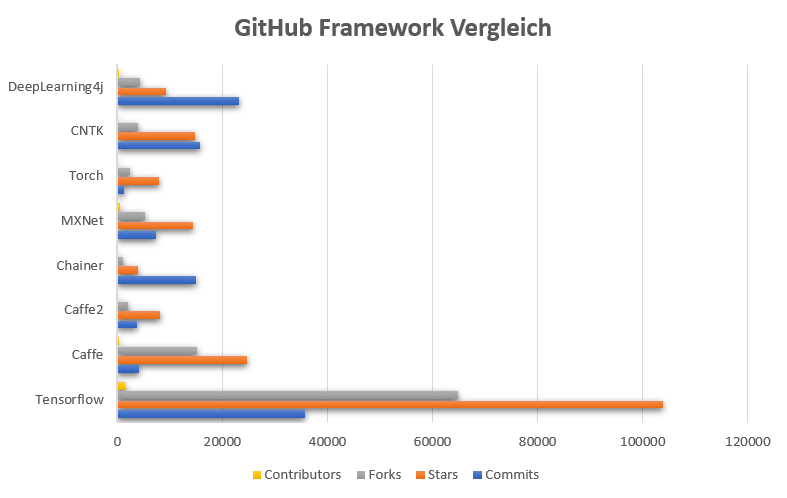
\includegraphics[width=0.9\linewidth]{Pictures/GitHubFrameworkVergleich}
	\caption[GitHub: Vergleich des Interesses in verschiedene Deep Learning Frameworks]{GitHub: Vergleich des Interesses an o.g. Deep Learning Frameworks}
	\label{fig:githubinterestdeeplearning}
\end{figure}
